\section{Массы и энергии связи нейтроноизбыточных изотопов} \label{massmodel}
Массы взаимодействующих и результирующих частиц являются важнейшими параметрами расчета сечений ядерной реакции при помощи статистической модели. В частности, энергия связи ядра используется при расчете плотности высоколежащих уровней, которая в модели Ферми-газа задается формулой
\begin{equation} \displaystyle
  \omega(E) = \frac{\sqrt{\pi}}{12} 
  \frac{\exp [ 2\sqrt{a(E-\Delta)} ] }
       {a^{1/4}(E-\Delta)^{5/4}},
\end{equation}
где $a$ и $\Delta$ являются параметрами модели, а $E$ есть энергия возбуждения системы. В случае реакции нейтронного захвата энергия возбуждения $E$ равна сумме кинетической энергии нейтрона и энергии его отделения $S_n$, которая в свою очередь определяется как разница энергий связи $B(N,Z)$ конечного и исходного изотопа:
\begin{equation}
S_n = B(N, Z) - B(N - 1, Z)
\end{equation}

При этом, как видно из работы~\cite{sobiczewski2018}, предсказания масс экзотических изотопов при помощи различных ядерных моделей существенно различаются между собой. Важно исследовать влияние этих неопределенностей на расчеты сечений астрофизических ядерных реакций и на результаты моделирования $r$-процесса. Для этого мы рассмотрим три модели, позволяющие рассчитывать массы ядер и использующие разные подходы.

По методу описания ядерной материи теоретические модели делятся на коллективные, или макроскопические, и микроскопические. Коллективный подход, к которому относится, например, известная формула Вайцзеккера, рассматривает ядро как единое целое, например, как каплю несжимаемой жидкости. В его пользу свидетельствуют деформации ядер, колебательные и вращательные полосы в спектрах. При необходимости описать более тонкие одночастичные эффекты прибегают к микроскопическим моделям, а также коллективным моделям с микроскопическими поправками. Микроскопические модели зачастую основаны на принципе эффективного потенциала, сводящем задачу взаимодействия многих тел к задаче невзаимодействующих тел в общем потенциале.

Для расчета астрофизических скоростей реакций мы используем результаты трех ядерных моделей, реализующих разные подходы к описанию ядерной материи: макро-микроскопической модели FRDM2012~\cite{moller2016}, микроскопической модели HFB-24~\cite{goriely2013} и феноменологического метода локальных массовых соотношений LMR2021~\cite{vladimirova2022}. Настоящий раздел посвящен их обзору и сравнению.

\input tex/pt2_masses/frdm.tex
\input tex/pt2_masses/hfb.tex
\input tex/pt2_masses/lmr.tex

\subsection{Заключение}
Описанные в настоящем разделе ядерные модели использовались нами для расчета скоростей реакций нейтронного захвата, участвующих в астрофизическом $r$-процессе.Выбор именно этих моделей обусловлен тем, что каждая из них реализует отдельный подход к предсказанию масс экзотических ядер. Будет интересно посмотреть, как различные методы расчета ядерных масс влияют на результаты моделирования $r$-процесса.

\begin{figure}
  \centering
  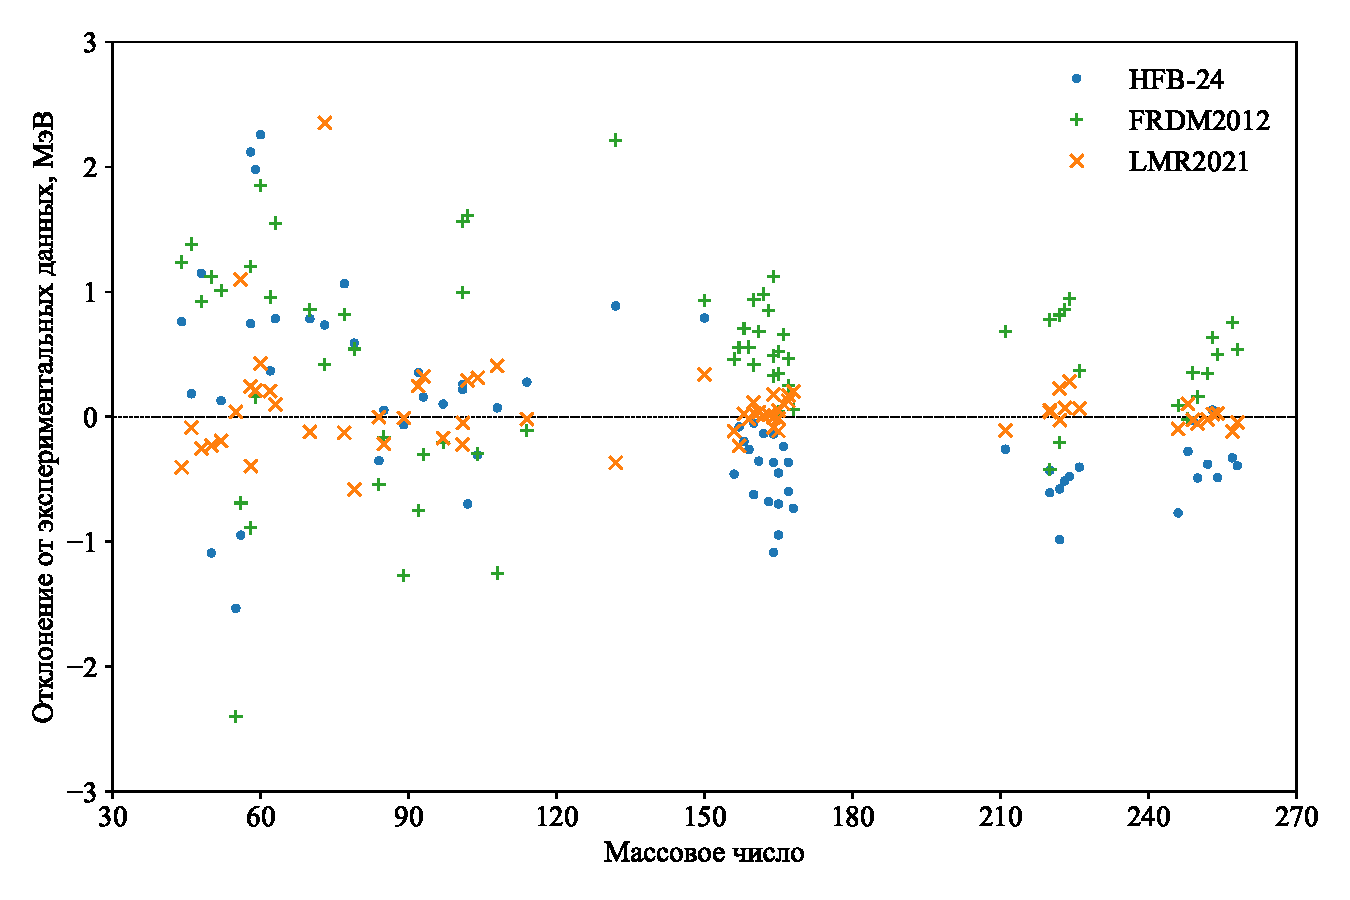
\includegraphics[width=0.9\textwidth]{pics/deviations.pdf}
  \caption{Разница теоретических энергий связи из таблиц FRDM2012~\cite{moller2016}, HFB-24~\cite{goriely2013} и специальной версии LMR2021~\cite{vladimirova2022} (см.пояснение в тексте) и экспериментальных значений из базы данных AME2020~\cite{huang2021}.}
  \label{fig:deviations}
\end{figure}

Для нас наиболее интересны предсказания масс изотопов с большим избытком нейтронов, которые не могут быть получены в лабораторных условиях. Оценить точность теоретических моделей в этой области $NZ$-диаграммы не представляется возможным в силу отсутствия экспериментальных данных. Тем не менее можно проанализировать точность предсказания моделей вблизи долины стабильности. Для этого мы исследовали отклонения теоретических энергий связи от экспериментальных значений из базы данных AME2020 для ряда ядер. При этом в качестве таблицы LMR2021 использовалась специальная версия, рассчитанная описанным выше методом, но на основе базы данных AME2016, а не более новой AME2020. Использование именно этой версии таблицы обусловлено тем, что в массовую таблицу LMR2021 исходные экспериментальные данные входят без изменений, поэтому сравнивать стандартную версию таблицы с AME2020 было бы некорректно.

На рис.~\ref{fig:deviations} представлены результаты этого сранения. Среднеквадратичные отклонения составляют $0.73$~МэВ для HFB-24, $0.89$~МэВ для FRDM2012 и $0.37$~МэВ для специальной версии LMR2021. Как видно, для новых экспериментальных данных, появившихся в последней версии AME2020
предсказания всех трех моделей имеют значительные флуктуации в области легких ядер. Для массовых чисел $A > 120$ модель FRDM2012 заметно завышает, а HFB-24 занижает величину энергии связи. Метод локальных массовых соотношений LMR2021 при этом обладает наивысшей точностью. Это может быть связано с тем, что методом LMR2021 коллективные и микроскопические эффекты учитываются неявно за счет исходных экспериментальных данных, не делается никаких сильных предположений о структуре и физике ядер. 

Однако точность предсказаний на малом удалении от долины стабильности не гарантирует ее сохранение в области сверхнейтроноизбыточных изотопов, где в основном протекает $r$-процесс. Безусловно для развития понимания астрофизического $r$-процесса и нуклеосинтеза в целом необходимо совершенствовать наши представления о физике нейтроноизбыточных ядер.

